% !TeX spellcheck = de_DE
% !TeX encoding = UTF-8
% !TeX spellcheck = en_US
% !BIB TS-program = biber
% basic packages and document settings
\documentclass[a4paper,12pt]{article}
\usepackage[english]{babel}
\usepackage[utf8]{inputenc}
\usepackage[T1]{fontenc}
\usepackage[a4paper]{geometry}
\geometry{top = 30mm, bottom = 25mm, left = 25mm, right = 25mm}
\usepackage{setspace}
\onehalfspacing
\raggedbottom
\pdfcompresslevel9

% mathmode-related packages
\usepackage{mathtools}
\usepackage{physics}
\usepackage{amsmath}
\usepackage{amsthm}
\usepackage{amsbsy}
\usepackage{mathrsfs}
\usepackage{amssymb}
\usepackage{amstext}
\usepackage{amsfonts}
\usepackage{tikz}
\usepackage{siunitx}
%\usepackage{IEEEtrantools}

% misc
\usepackage{esdiff}
\usepackage{multirow}
\usepackage{blindtext}
\usepackage{todonotes}
\usepackage{abstract}
\usepackage{appendix}
\usepackage[bottom]{footmisc}
\usepackage{listings}
\usepackage{dashrule}

% graphics and floats
\usepackage{graphicx}
\graphicspath{{../Figures/}}
\usepackage{tikz}
\usepackage{float}
\usepackage{wrapfig}
%\usepackage{subfloat}
\usepackage{subcaption}
%\usepackage{caption}
\usepackage[rightcaption]{sidecap}
\usepackage{tabularx}
\usepackage{adjustbox}
%\usepackage{svg}
\usepackage{epstopdf}
\usepackage{grffile}	% handle file names with dots, spaces etc.
%\usepackage{flafter}
\usepackage{rotating}
%\usepackage{floatrow}
%\floatsetup[figure]{capposition=beside,capbesideposition={top,right}}

%\usepackage{epstopdf}
%\epstopdfDeclareGraphicsRule{.pdf}{png}{.png}{convert #1 \OutputFile}
%\AppendGraphicsExtensions{.pdf}

% packages requiring setup arguments

\usepackage{xcolor}
%\definecolor{rwth-dark}{HTML}{176daf}
\definecolor{rwth-dark}{RGB}{0,84,159}
%\definecolor{rwth-light}{HTML}{8abae3}
\definecolor{rwth-light}{RGB}{142,186,229}

%/**
%* Generated by Gpick 0.2.5
%* RWTH Dark: #176daf, rgb(23, 109, 175), hsl(32, 43%, 69%)
%* RWTH Light: #8abae3, rgb(138, 186, 227), hsl(195, 73%, 89%)
%*/

\usepackage{hyperref}
\hypersetup{hidelinks=true,colorlinks=true,allcolors=rwth-dark}
\usepackage[nameinlink,capitalise]{cleveref}
%\usepackage[hyphens]{url}
%\urlstyle{sf}
%\usepackage{breakurl}


% header & footer settings
\usepackage{fancyhdr}
\pagestyle{fancy}
%\renewcommand{\chaptermark}[1]{\markboth{#1}{}} % with this we ensure that the chapter and section headings are in lowercase.
\renewcommand{\sectionmark}[1]{\markright{\thesection\ #1}}
\fancyhf{} % delete current header and footer

%\fancyhead[LE,RO]{\large\thepage}
\fancyhead[L]{\large\rightmark}
\fancyhead[R]{\large\thepage}

\renewcommand{\headrulewidth}{0.3pt}
\renewcommand{\footrulewidth}{0pt}
%\addtolength{\headheight}{0.5pt} % space for the rule

\fancyfoot[C]{\thepage}

\fancypagestyle{plain}
{
	\fancyhead{} % get rid of headers on plain pages
	\renewcommand{\headrulewidth}{0pt} % and the line
}

% ========== command definitions =================================
\newcommand{\Thickline}{\rule{\linewidth}{0.4mm}}
\newcommand{\Thinline}{\rule{\linewidth}{0.1mm}}

\newcommand{\id}{\, \mathrm{d}}

\definecolor{codegray}{gray}{0.9}
\newcommand{\code}[1]{\colorbox{codegray}{\texttt{#1}}}

\newcommand{\skippage}{\clearpage{\thispagestyle{empty}\cleardoublepage}}

\def\@esphack{%
	\relax
	\ifhmode
	\spacefactor\@savsf
	\ifdim\@savsk>\z@
	\ignorespaces
	\fi
	\fi}

\title{\LARGE title}
\date{}


\begin{document}
	
\begin{titlepage}
	\thispagestyle{empty}
	\newgeometry{top=20mm, left=20mm, right=20mm, bottom=20mm}
	
%	\begin{minipage}{0.35\textwidth}
%		\begin{flushleft}
%
%
%		\end{flushleft}
%	\end{minipage}
%	\hfill
%	\begin{minipage}{0.65\textwidth}
%		\begin{flushright}
%
%		\end{flushright}
%	\end{minipage}
	
%	\vspace*{\fill}
	\hspace{0pt}
	\vspace{2cm}
	\begin{center}
%		\Thickline
%		\vskip -0.5cm
%		\Thinline
		\hdashrule{\linewidth}{1pt}{}
		\vskip -0.5cm
		\hdashrule{\linewidth}{0.5pt}{}
		
		\vspace{0.5cm}
		\Huge{ \textbf{ T7 \\}}
		\LARGE{ \textbf{Gaseous ionisation detectors and statistics} } 
		
		\hdashrule{\linewidth}{0.5pt}{}
		\vskip -0.95cm
		\hdashrule{\linewidth}{1pt}{}
%		\Thinline
%		\vskip -0.9cm
%		\Thickline 
		
		\vspace{3cm}
		\Large{\textbf{ Group 14 \\}}
		\Large{Heithem Assili, 368441 \\ Alexandre Drouet, 355095 \\ Olexiy Fedorets, 356615 \\}
		\vspace{1cm}
		\Large{\textsl{ Date of experiment: 14.03.2019 \\ Submission date: 28.03.2019}}
		
	\end{center}
	\vfill
%	\vspace*{\fill}
	
\end{titlepage}
	
	
	
%\skippage
\pagenumbering{roman}
\thispagestyle{plain}

\tableofcontents
%	\newpage
\newpage
\listoffigures

%\begingroup
%\let\cleardoublepage\relax
%\let\clearpage\relax
\listoftables
%\endgroup
%\listoftables

\skippage

\pagenumbering{arabic}
\setcounter{page}{1}
\restoregeometry
\thispagestyle{fancy}


\section{Introduction}

The goal of this experiment is to get aquainted with gas detectors and to learn how to operate them. Furthermore we want to measure statistical distributions related to decay processes.

\subsection{Gas detectors}

\subsection{Statistics}

\section{Measurments with the Geiger counter}

\subsection{Procedure}

First we placed a Sr90-Probe in a lead chamber and measured the count rate's dependence on the voltage. 

\subsection{Analysis}
\subsection{Characterization of dead time}

First of all we generate a Plus of $1\,MHz$ with the Generator
that is linked to the variable totzeitstufe($2\,ms$,$1\mu\,s$) and write the counts down(counts over $2\,s$ measured $3$ times).
With
\begin{equation}
N =\frac{n}{1-n\cdot\tau}=\frac{n}{1-n\cdot\tau}
\end{equation}
 we can corrtect the Stufe if we consider that the smaller stufe is correct 
with a measured countrate of $10^6$ for $1\mu\,s$ and 
$519.67\pm0.07$ for $2\,ms$ we get a corrected stufe of $1.92\,ms$

now we can calculate with the same method the auflösungszeit of the GM-Counter.
we consider that the real stufe is between $1\mu\,s$ and $2\,ms$ 

with 
\begin{equation}
\tau =\frac{1}{n}-\frac{1}{n}+\tau
\end{equation}
 ,$n=179.6\pm0.6\,\frac{1}{s}$ and$n=246.0\pm1.8\,\frac{1}{s}$ we got a auflösungszeit of $\tau=422\pm35\,ms $
.
\subsection{Stever-Diagramm}

\begin{figure}[H]
\centering
\includegraphics[width=\textwidth]{../Figures/Steverdiag.jpg}
\caption{Stever-Diagramm}
\label{fig:Stever-Diagramm}
\end{figure}
with a stever we  can estimate the auflösungszeit on the oscilliscope out of the dead time an the relax time that we can read from the scope 

the deadtime is the distance between the main peak and the next incoming peak, during that time the GM-Counter can not detect anything.
 We estimate the dead time with $224\pm4\mu\,s$ (for that we read the dead time out of the steverdiagram 3 time with a min and max value and mean over all)
 The realaxtime is the distance bewteen main peak and the next main peak , therfore we got  $505\pm11\mu\,s$ (same method as before)  
 
\subsection{Characteristic curve of GM-Counter}
after the dead time correcture we can now study the Characteristic Geiger-Curve.
We Plot the Voltage(in 10 Volt steps) over the measured Counts in 1s ($\frac{Counts}{10\,s}$.

with the calculated auflösungszeit we can now correct the Characteistic GM-Curve for the detected count with $N =\frac{n}{1-n\cdot\tau}$ 
for errors we used gaussian propagation of uncertainty 


\begin{figure}[H]
\centering
\includegraphics[width=\textwidth]{../Figures/Geiger_characteristic_curves_with_deadcorect.pdf}
\caption{GM-Characteristic}
\label{fig:GM-Characteristic}
\end{figure}



\section{Measurement of statistical distributions}

\subsection{Procedure}

First we set the measurement, such that an average of at least 25 events were recorded per measurement, while the Sr-probe was in the detector. We found $10\,s$ to be a good interval. Then we measured the number of events per $10\,s$, 100 times.

Next we removed the probe from the chamber and set the measurement time, such that the average event count per measurement was at most 2. There we found $2\,s$ to be a good intervall. Then we measured the number of events per $2\,s$, 111 times

Next we placed the probe in the chamber again and used the oscilloscope to take a shot of the pulses on a $50\,ms$ scale. We will use this data to measure the times between two consecutive events.

We repeated the last measurement with an alternative method: using the counter we recorded the counts per $0.1\,s$ 50 times.

\subsection{Analysis}

In \cref{fig:GaussHist} we see the recorded count rates for the Geiger counter with the Sr-probe in a histogramm, that vaguely resemble a gaussian distribution. We calculated the mean and standard deviation of our data and with those calculated our expected gauss distribution, according to
\begin{equation}
P(k) = \frac{1}{\sqrt{2\pi}\sigma} \exp(-\frac{(k-\mu)^2}{2\sigma^2}).
\end{equation}
This expected curve is shown in \cref{fig:GaussFit} together with the normalized histogramm of the count rates. In the same figure we also plotted a gauss curve we fitted with the least square method with $\mu$ and $\sigma$ as free parameters.

\begin{figure}[H]
\centering
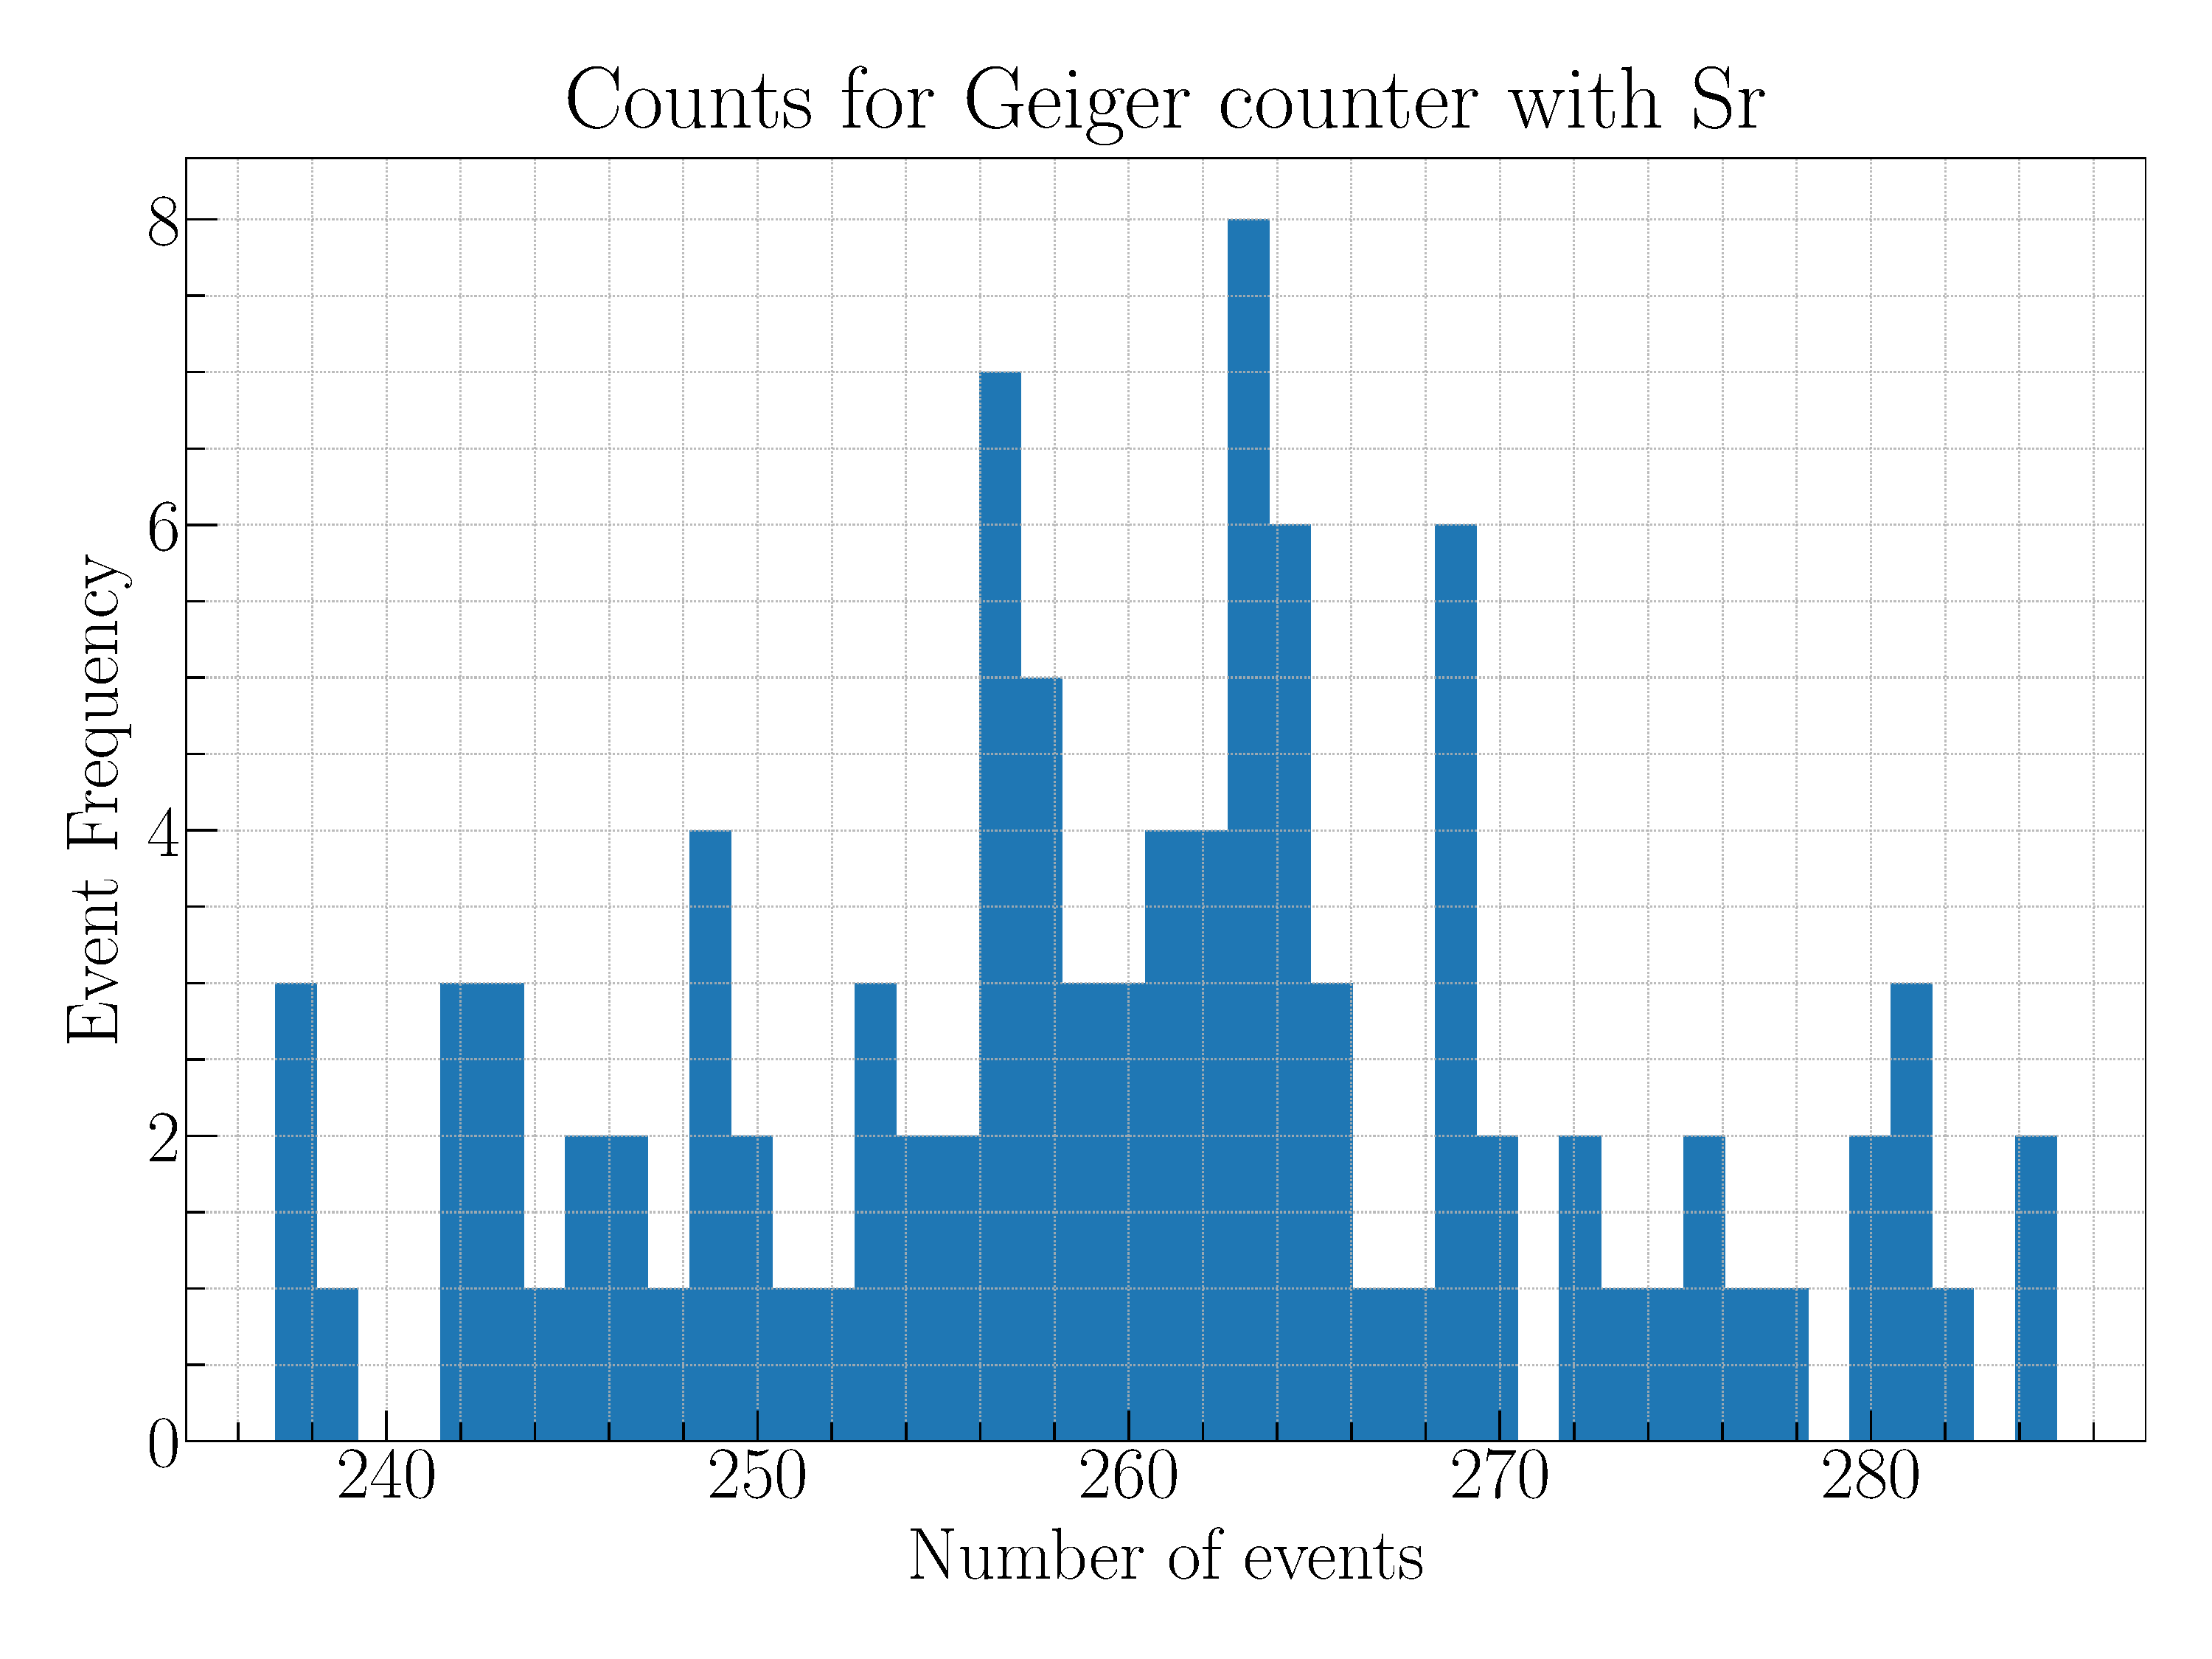
\includegraphics[width=\textwidth]{../Figures/Geiger_gauss_histogram.pdf}
\caption{gauss hist}
\label{fig:GaussHist}
\end{figure}

\begin{figure}[H]
\centering
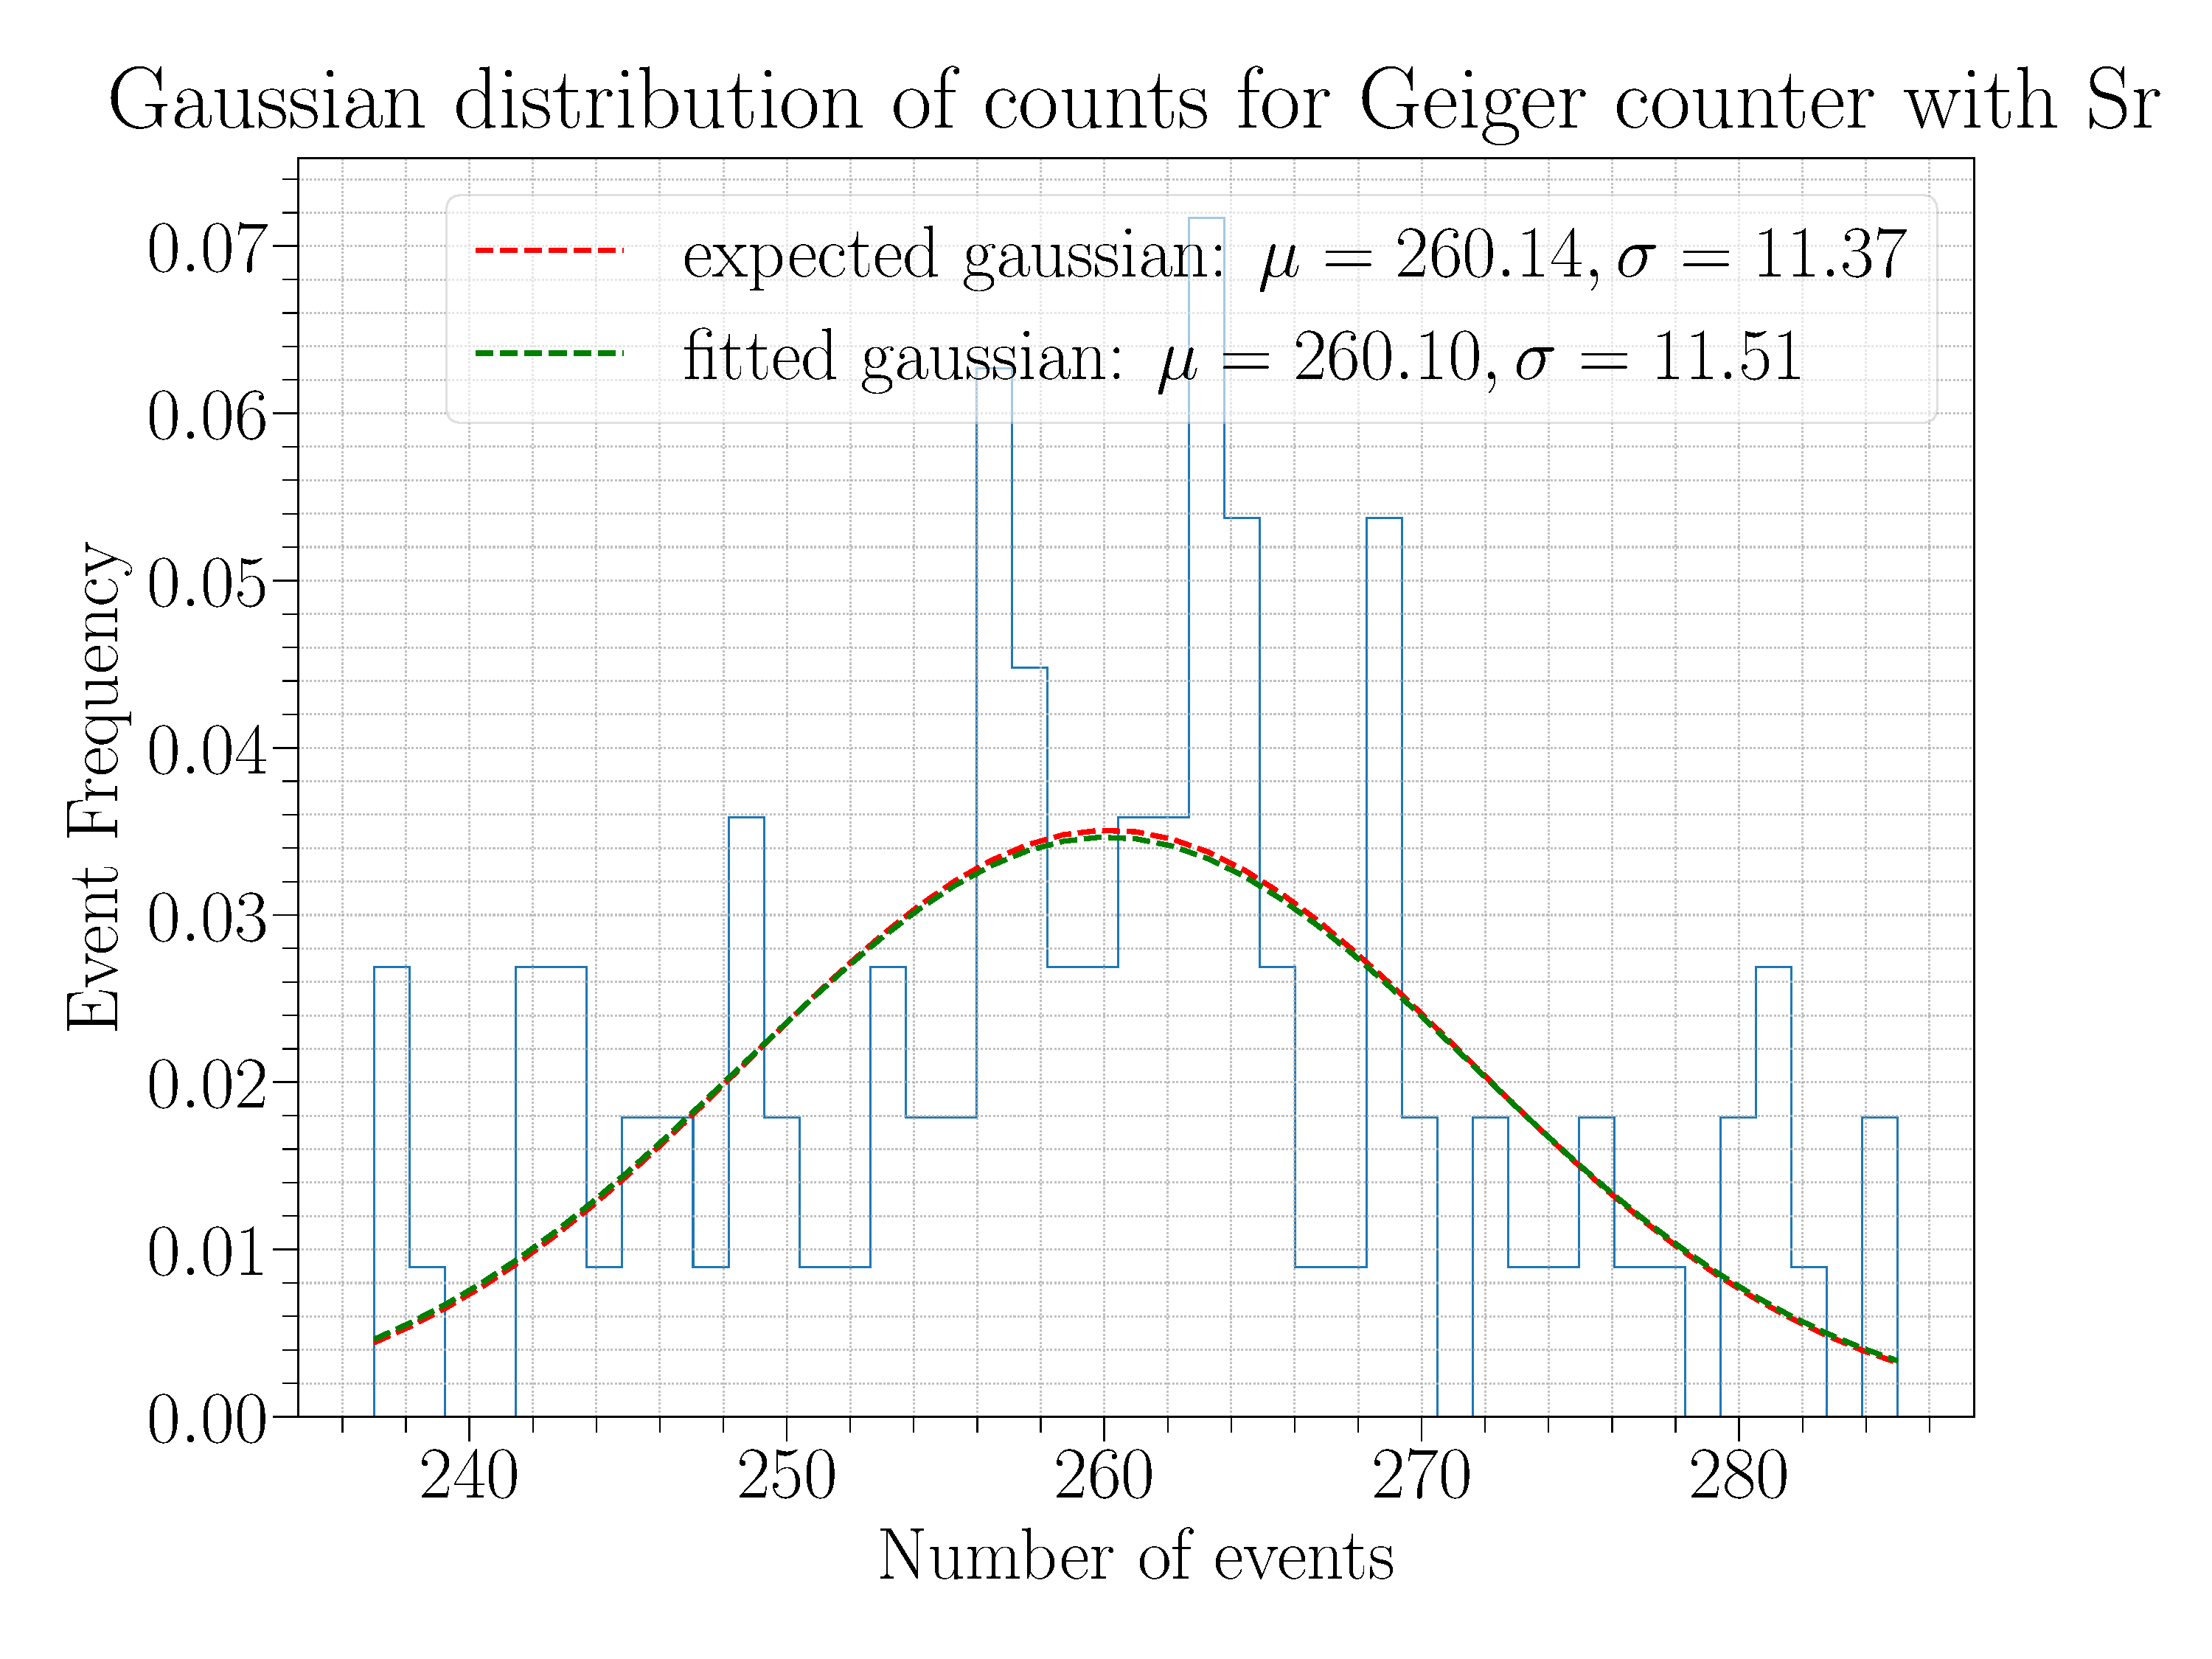
\includegraphics[width=\textwidth]{../Figures/Geiger_gauss_fit.pdf}
\caption{gauss fit}
\label{fig:GaussFit}
\end{figure}

We proceed analogously for the count rates of the empty Geiger counter. In \cref{fig:PoissonHist} we see the measured count rates and in \cref{fig:PoissonFit} we plotted the normalized histogramm, together with both the expected and the fitted poisson distribution
\begin{equation}
P(k) = \frac{\mu^k e^{-\mu}}{k!}.
\end{equation}
Of course here we only have one parameter, the mean value $\mu$, since the standard deviation is given by $\sigma = \sqrt{\mu}$.

\begin{figure}[H]
\centering
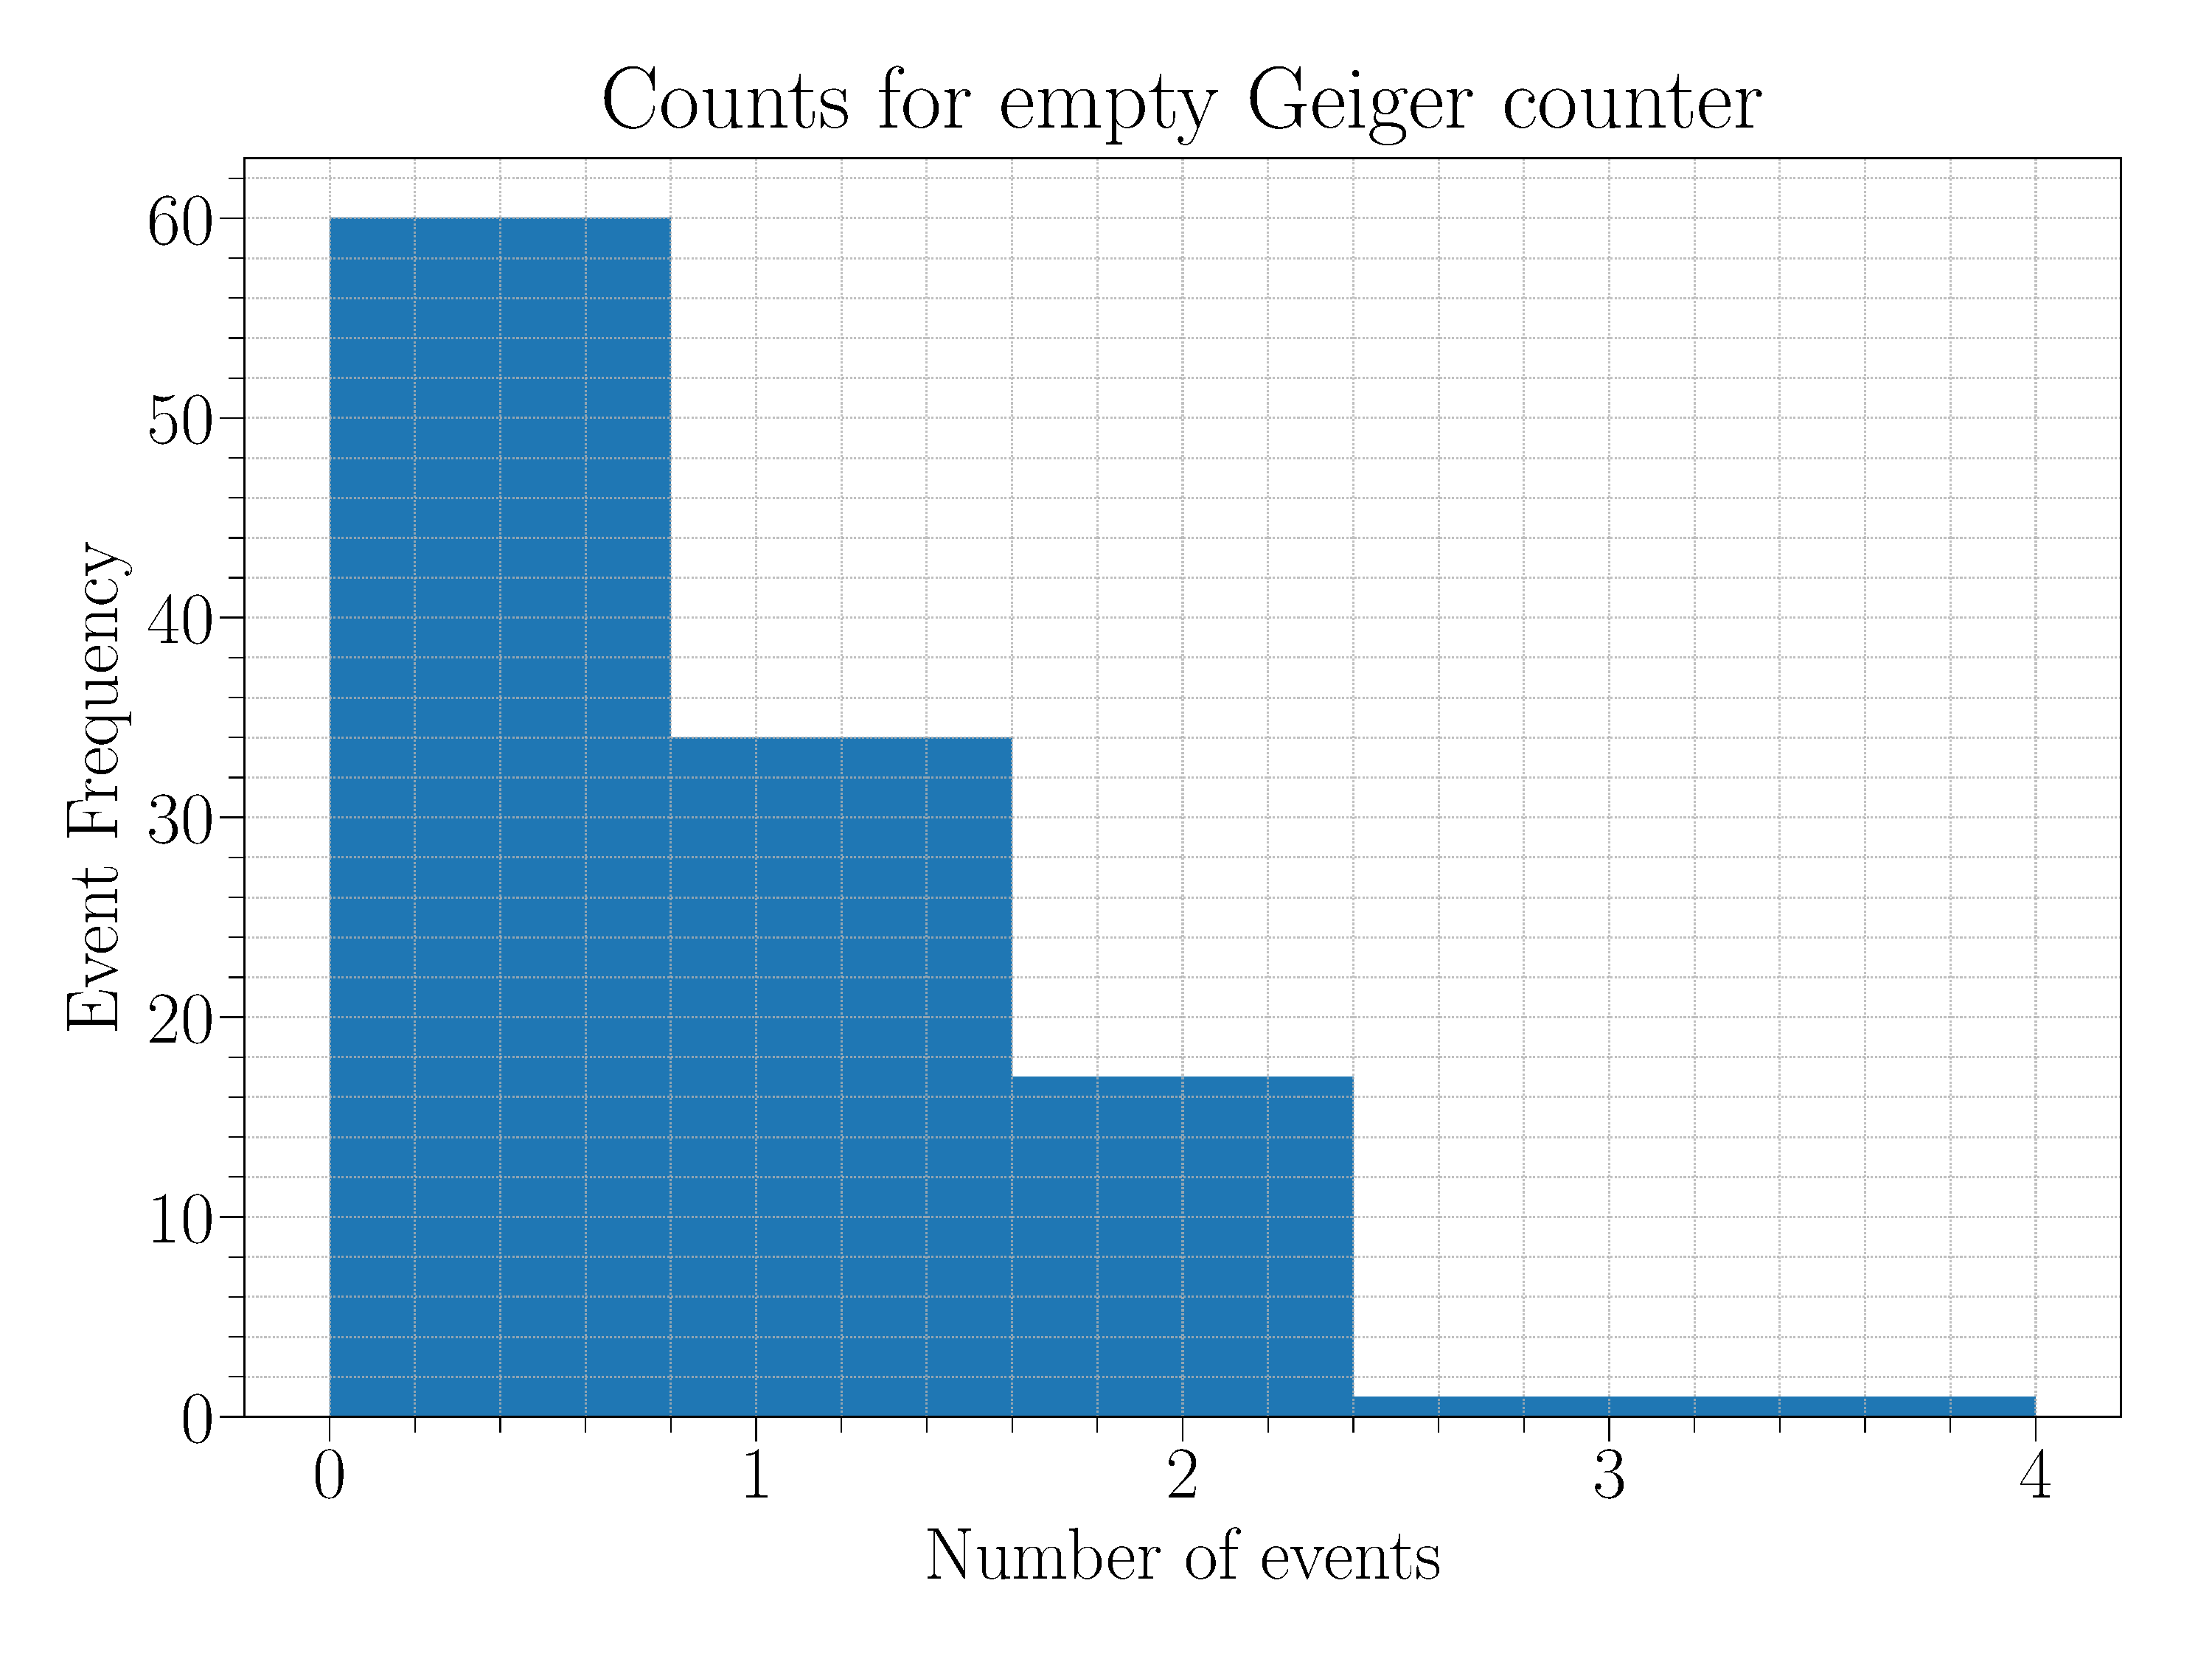
\includegraphics[width=\textwidth]{../Figures/Geiger_poisson_histogram.pdf}
\caption{poisson hist}
\label{fig:PoissonHist}
\end{figure}

\begin{figure}[H]
\centering
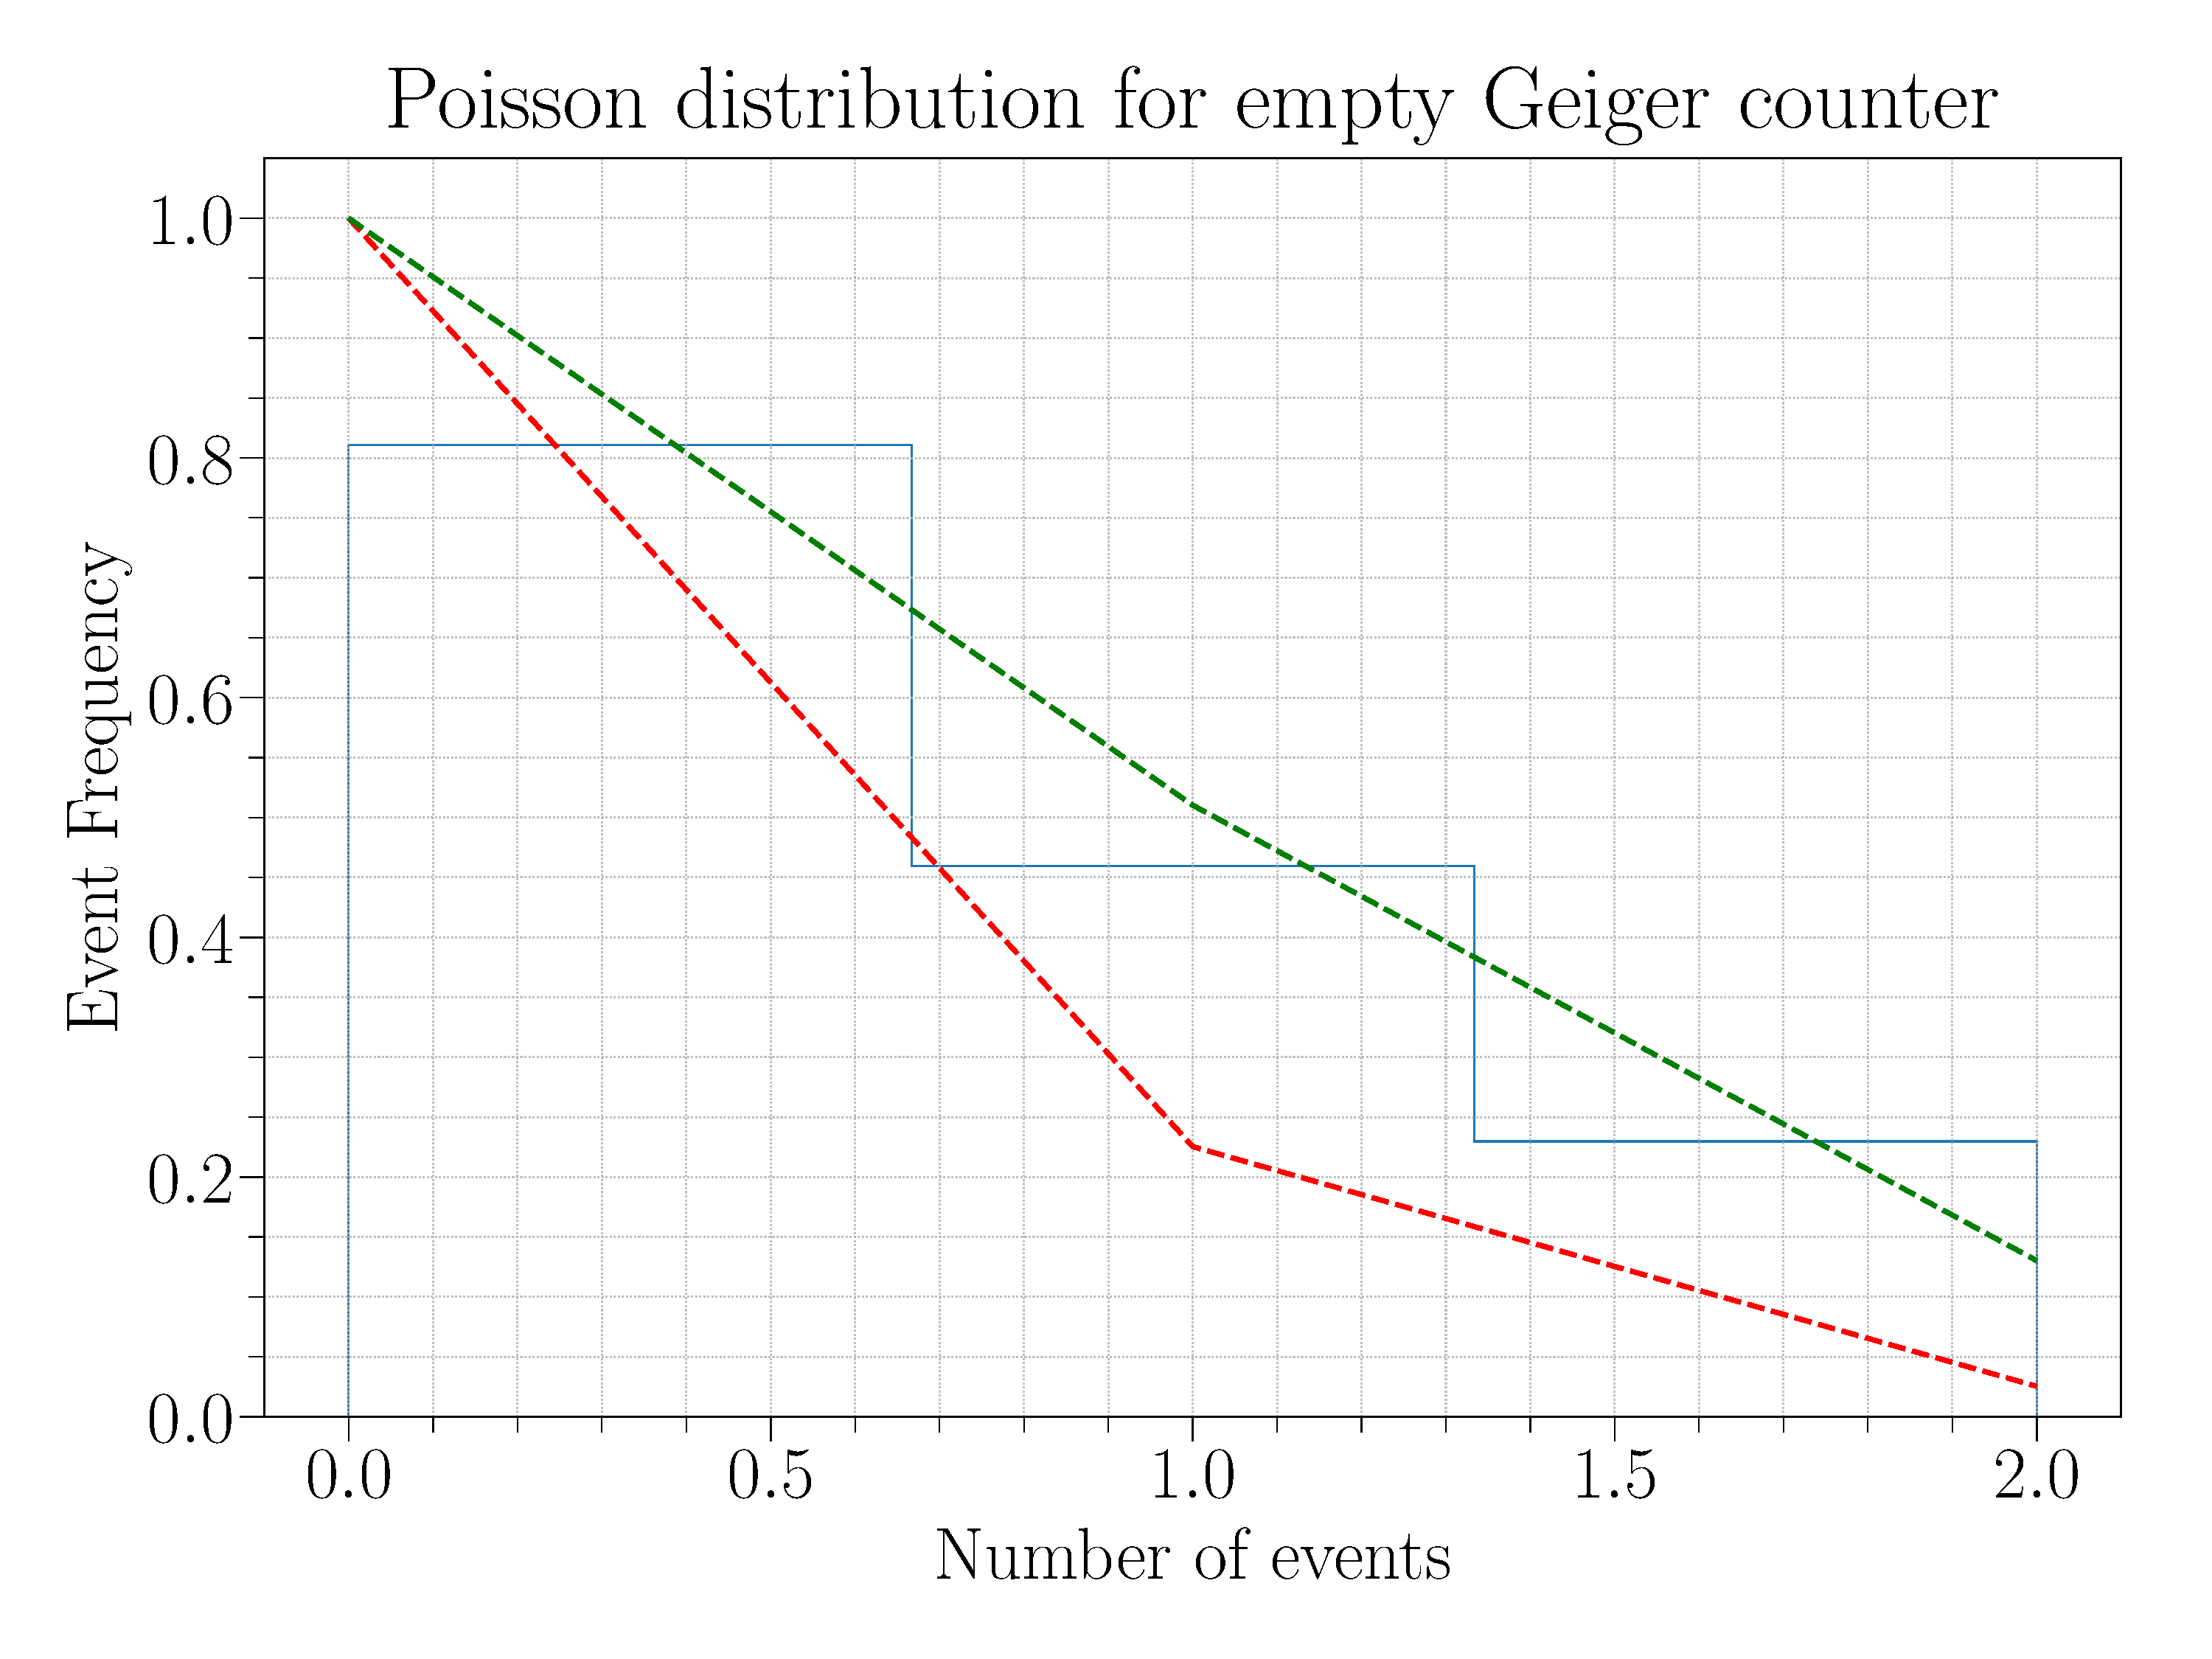
\includegraphics[width=\textwidth]{../Figures/Geiger_poisson_fit.pdf}
\caption{poisson fit}
\label{fig:PoissonFit}
\end{figure}

TODO: chi2 test und tabelle mit ergebnissen

To test the goodness of our predictions, we did a $\chi^2$ test for all of the distributions.  

\section{Measurements with the proportional counter}

\subsection{Procedure}

\subsection{Analysis}

\section{Conclusion}



\end{document}
